\chapter{Propuesta de solución}
\label{cap:propuesta-de-solucion}

El objetivo del \gls{tfg} consiste en desarrollar un sistema que reconstruya un cuerpo humano completo, utilizando como sensor para la adquisición de los datos el Intel RealSense D435 y el sistema embebido Jetson Nano como computador que procesará los datos en la fase de registro.
Por ello, en este capítulo detallaremos cuales han sido los pasos a seguir para conseguir un sistema que funcione y sea capaz de llevar a cabo esta reconstrucción.

En la Figura \ref{fig:diagrama-propuesta-solucion} podemos ver un diagrama de la implementación de los módulos del sistema, desde la fase de adquisición, pasando por la fase de registro, hasta la fase de análisis con los resultados finales.

\begin{figure}[h]
    \centering
    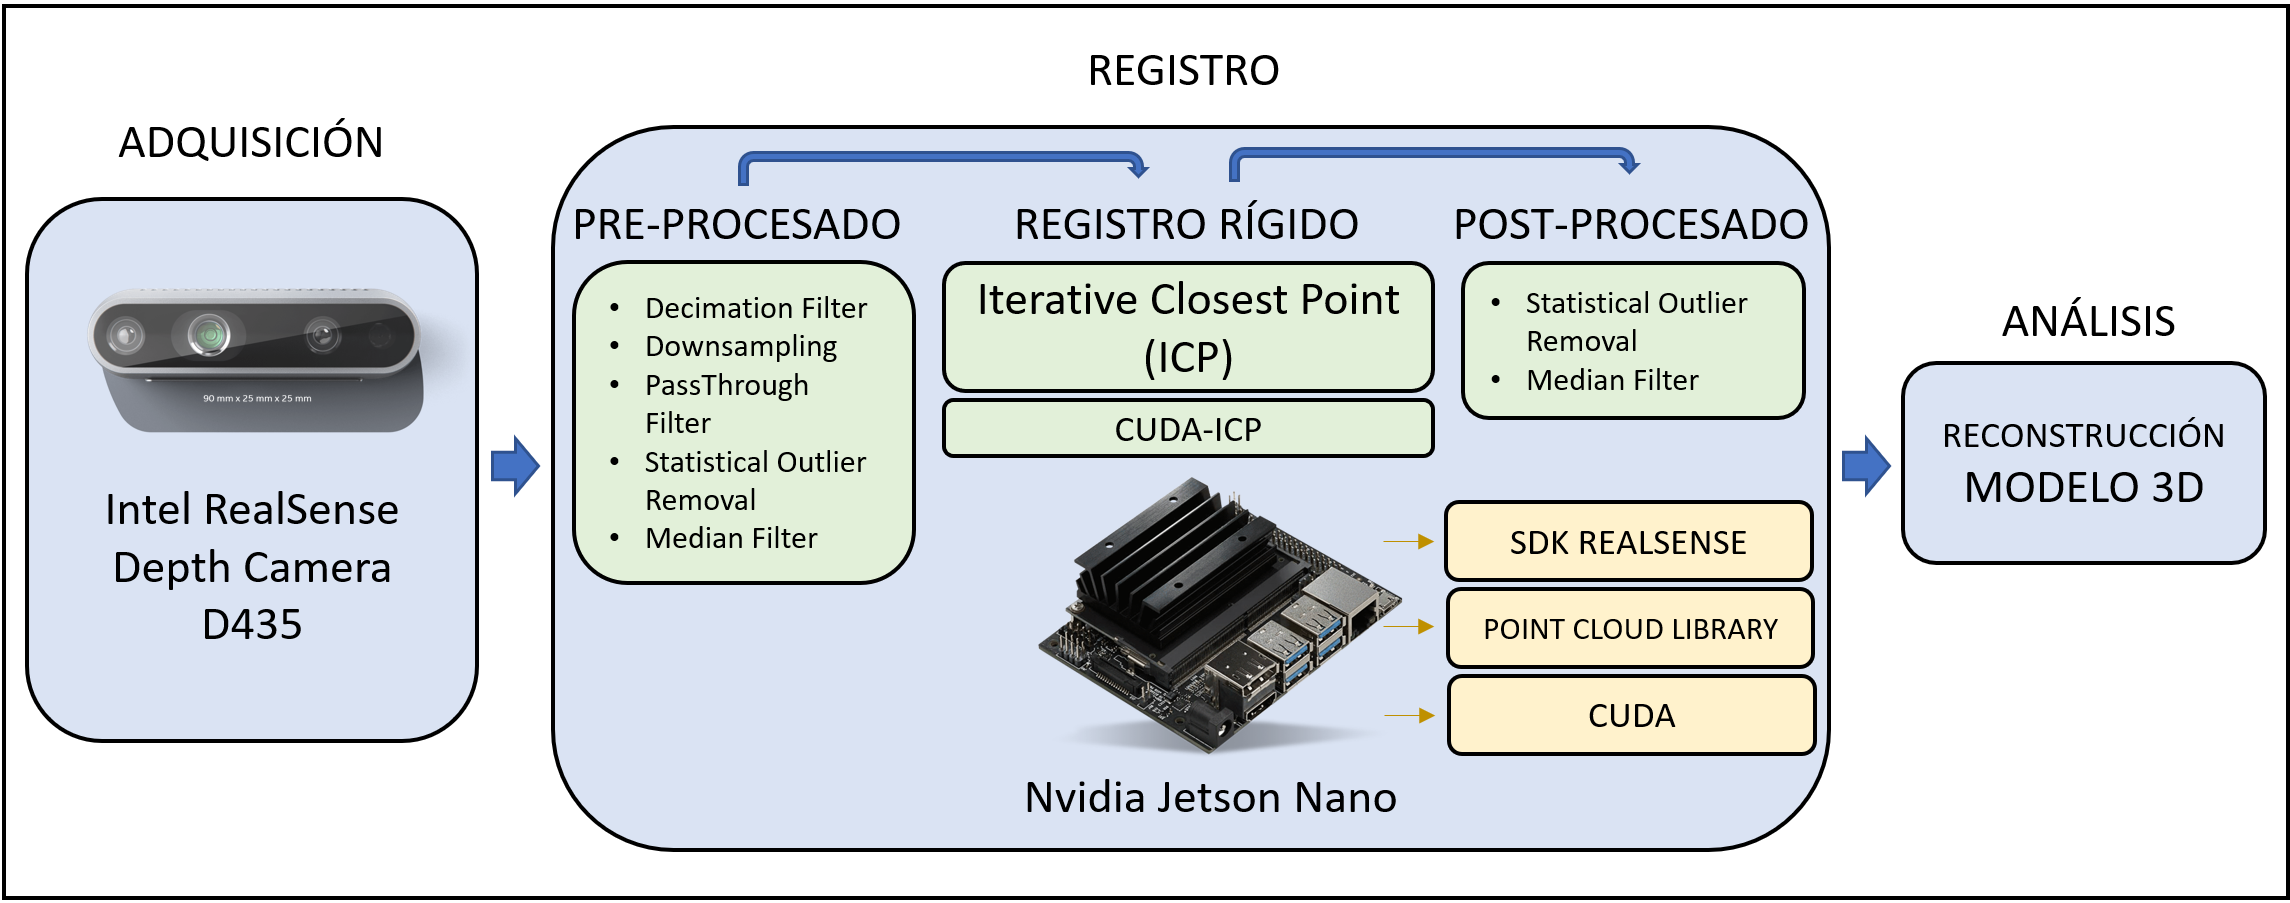
\includegraphics[width=\textwidth]{archivos/diagrama-propuesta-solucion.png}
    \caption{Diagrama de la propuesta e implementación de los módulos del sistema.}
    \label{fig:diagrama-propuesta-solucion}
\end{figure}

A continuación, durante este capítulo desarrollaremos cada una de las partes del diagrama explicando las cosas implementadas y el funcionamiento de cada uno de los módulos.

\section{Adquisición de datos}

Nuestro sistema de reconocimiento \gls{3d} consta del sensor Intel RealSense D435 conectado directamente a través de un puerto USB 3.0 al dispositivo Nvidia Jetson Nano.

Durante la fase de adquisición, el objetivo será realizar capturas RGBD a un modelo a través del sensor Intel RealSense D435.
Para ello, el sensor deberá estar fijo y el modelo deberá estar situado en el centro de la imagen para una mayor nitidez en las capturas.
El sensor realizará capturas constantemente y consecutivamente, mientras el modelo rota 360º poco a poco.
De esta forma, obtendremos muchas capturas desde distintos ángulos del modelo que posteriormente se procesarán para ser alineadas y reconstruir el modelo completamente en \gls{3d}.

Por tanto, será importante tener en cuenta la frecuencia de capturación del sensor, ya que cuanto mayor frecuencia, más rápido capturará al modelo, y menor será el ángulo de rotación entre cada una de las capturas.
Esto quiere decir que la distancia entre los puntos de dos capturas consecutivas será muy pequeña, y facilitará la tarea del registro con el algoritmo \gls{icp}.

El sensor Intel RealSense D435 es capaz de capturar a una frecuencia de hasta 30Hz en modo RGBD.
Realmente esto es más que suficiente, ya que 30Hz quiere decir que es capaz de capturar 30 imágenes en un segundo.
Hemos definido que cuanto más rápido se realicen las capturas es mejor, pero tanta velocidad realmente puede llegar a ser perjudicial, debido a que a esa frecuencia pueden llegar a realizarse cientos de capturas hasta que el modelo haya terminado de rotar 360º, haciendo que aumente el peso de trabajo a procesar debido a la enorme cantidad de datos.

Por ello, es necesario encontrar un punto medio. Como la frecuencia del sensor es mayor a las capturas que realmente queremos obtener por segundo, limitaremos la velocidad a la que se realizan las capturas introduciendo por parámetro un valor que indique cada cuanto realizar la captura.

Inicialmente y para testear, está bien separar la fase de adquisición de todas las capturas de la fase de registro. Sin embargo, se ha añadido una opción para funcionar de forma paralela e ir obteniendo el resultado a la vez que se realiza la adquisición total del modelo.
Es decir, una vez se hayan realizado la primera y segunda captura, estas serán enviadas para procesar el registro en otro hilo y, de forma concurrente, seguimos realizando la adquisición de nuevas capturas mientras el modelo está rotando.

\section{Pre-procesado}

Tras obtener la captura del modelo en la fase de adquisición, la captura se envía a la fase de pre-procesado donde se le aplicarán los filtros ya mencionados en apartados anteriores para reducir ruido y facilitar el procesamiento en la fase de registro.

El primer filtro a aplicar será el filtro diezmado (Decimal Filter). Este filtro realmente viene aplicado desde la fase de adquisición debido a que el filtro está integrado en la librería de RealSense desde la cual realizamos la captura, y se utiliza en el mismo proceso donde guardamos los datos y los enviamos al pre-procesado.
El filtro finalmente lo que consigue es una reducción de muestreo, como un downsampling, reduciendo el peso de la nube de puntos sin perjudicar demasiado la calidad, y facilitando las operaciones que se realizan dentro del algoritmo \gls{icp} que se procesará posteriormente.

Seguidamente al filtro de reducción de muestreo, se aplica el filtro ``Statistical Outlier Removal'' que nos permitirá deshacernos de los puntos atípicos que se encuentren más alejados del modelo en sí. Estos puntos normalmente son ruido por el borde del modelo que se genera en la fase de adquisición.
En la Figura \ref{fig:ejemplo-statistical-outlier-removal} podemos ver un ejemplo de aplicación de este filtro sobre un modelo \gls{3d}.

\begin{figure}[h]
    \centering
    \begin{subfigure}[t]{0.33\textheight}
    	\centering
        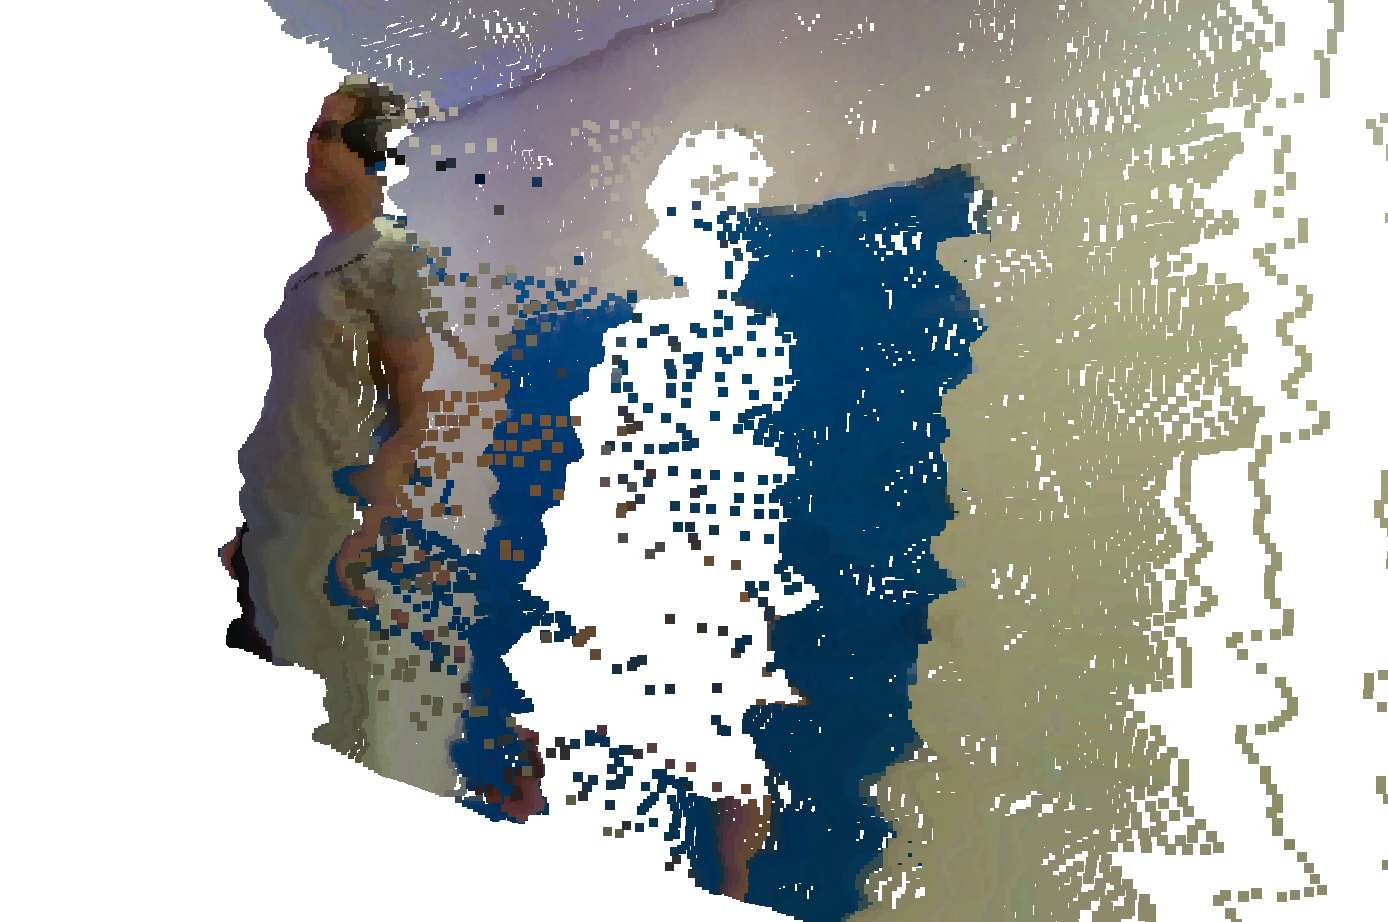
\includegraphics[height=4.5cm]{archivos/ejemplo-statistical-outlier-removal-original-2.png}
        \caption{Nube de puntos original.}
    \end{subfigure}
    \begin{subfigure}[t]{0.33\textheight}
    	\centering
        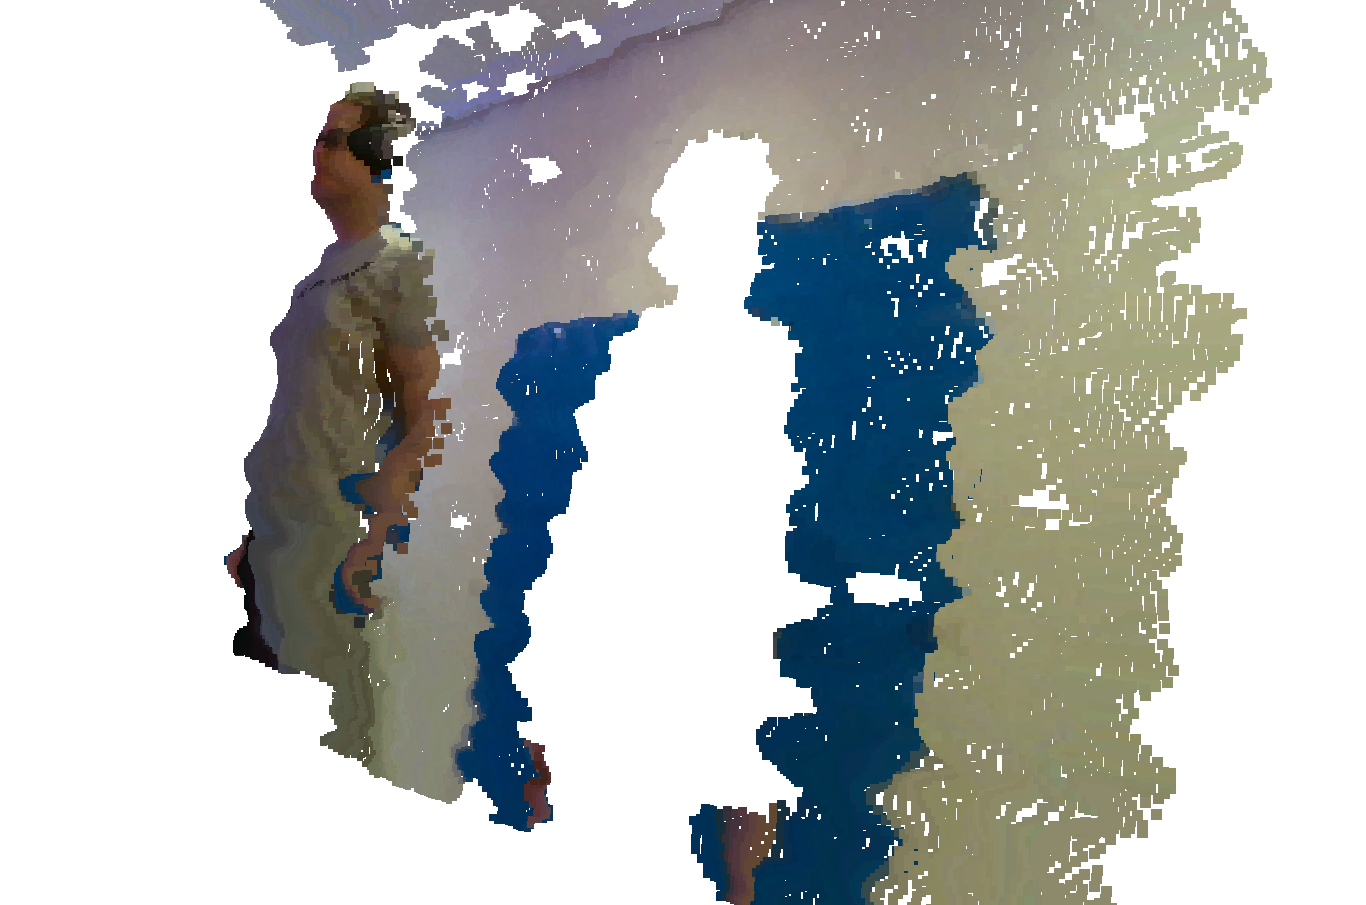
\includegraphics[height=4.5cm]{archivos/ejemplo-statistical-outlier-removal-filtro-2.png}
        \caption{Nube de puntos con filtro aplicado.}
    \end{subfigure}
    \caption{Ejemplo de filtro Statistical Outlier Removal aplicado.}
    \label{fig:ejemplo-statistical-outlier-removal}
\end{figure}

Por último, se aplica el filtro de la mediana, que permite homogeneizar el modelo \gls{3d} reduciendo el ruido que hay en el propio modelo, aplanandolo ligeramente.
% En la Figura \ref{fig:ejemplo-filtro-mediana} podemos ver un ejemplo de aplicación de este filtro sobre un modelo \gls{3d}.

% \begin{figure}[h]
%     \centering
%     \begin{subfigure}[t]{0.33\textheight}
%     	\centering
%         % 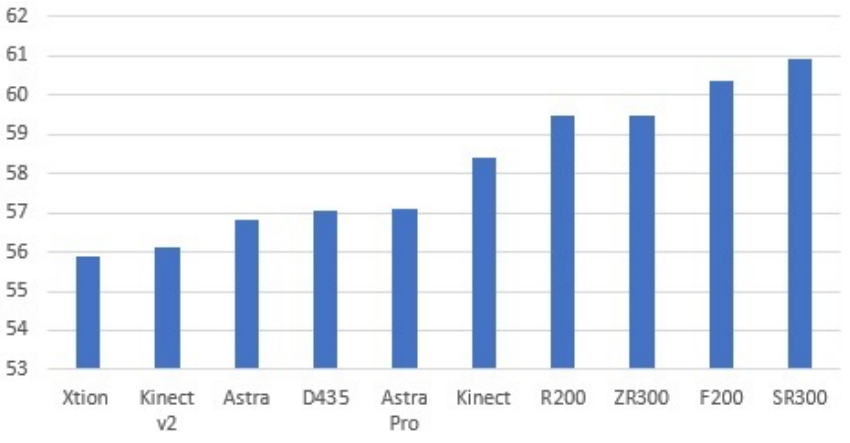
\includegraphics[height=3.5cm]{archivos/comparacion-sensores-recorrido1.png}
%         % la imagen debe ser con los puntos cercanos pero que sobre mucho de ambos lados sin corresponder, para mostrar que con el limite de maxima distancia esos puntos se ignorarian
%         \missingfigure{}
%         \caption{Nube de puntos original.}
%     \end{subfigure}
%     \begin{subfigure}[t]{0.33\textheight}
%     	\centering
%         % 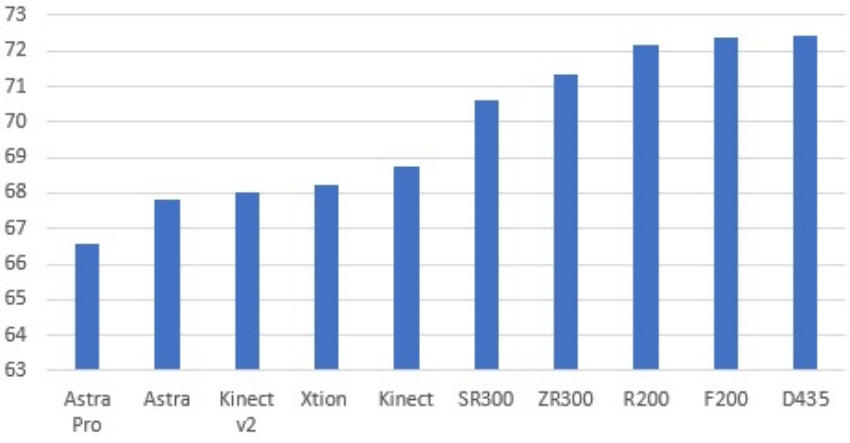
\includegraphics[height=3.5cm]{archivos/comparacion-sensores-recorrido2.png}
%         \missingfigure{}
%         \caption{Nube de puntos con filtro aplicado.}
%     \end{subfigure}
%     \caption{Ejemplo de filtro mediana aplicado.}
%     \label{fig:ejemplo-filtro-mediana}
% \end{figure}

\section{Registro}

En la fase de registro es donde conseguiremos reconstruir, poco a poco, el modelo en \gls{3d} por completo.
Para esta fase, nuestra solución consta de dos implementaciones sobre las que se han hecho las pruebas.
En una de ellas se utiliza el algoritmo \gls{icp} de la librería \gls{pcl}, y en la otra se utiliza CUDA-ICP, que se trata de una implementación en \gls{cuda} sobre el algoritmo \gls{icp} de la librería \gls{pcl} también.
No obstante, el uso de ambas implementaciones es el mismo, ambas reciben un modelo y una escena como entrada, y devuelven la matriz de transformación a aplicar sobre la escena.

Cabe destacar que no se hace uso de ningún algoritmo de grano grueso para un primer aproximamiento de la escena al modelo, como se ha explicado en la sección \ref{sec:metodos-de-registro}.
Aunque es muy común utilizar RANSAC-ICP para estos procesos de reconstrucción de modelos \gls{3d}, el caso de nuestro proyecto se encuentra muy bien definido en un entorno y unas características concretas que hacen que no sea necesario utilizar estos métodos como apoyo.
Debido a que la fase de adquisición es lo suficientemente rápida, la distancia entre cada par consecutivo de capturas es muy pequeña, lo cual nos permite procesar el método \gls{icp} sin necesidad de aproximar la escena previamente.

Por tanto, esta fase recibe dos nubes de puntos ya pre-procesadas, una de ellas será el modelo, y la otra será la escena.
En una primera iteración de esta solución, el algoritmo recibirá la captura 1 como la nube de puntos modelo, y la captura 2 como la nube de puntos escena.
Estas nubes de puntos son procesadas, obteniendo la matriz de transformación que hay que aplicar sobre la escena para que esta quede alineada con el modelo.
Seguidamente, transformamos la escena para que quede alineada con el modelo y juntamos ambas nubes de puntos, consiguiendo así una única nube de puntos que tenga la información de las capturas 1 y 2.
Nos guardamos la matriz de transformación obtenida para aplicarselo a las futuras escenas como matriz de transformación inicial.

En una segunda iteración de la solución, esta fase recibirá una nueva nube de puntos perteneciente a la captura 3, que será la nueva escena.
Por tanto, tendremos la nube de puntos modelo que constará de las capturas 1 y 2, y la nube de puntos escena que corresponde con la captura 3.
Previamente a procesar las nubes de puntos por el algoritmo \gls{icp}, se aplicará la matriz de transformación de la iteración anterior como transformación inicial para la captura 3, haciendo así que esta nube de puntos escena quede más próxima al modelo.
Ahora sí, las nubes de puntos serán procesadas por el algoritmo y obtendremos una nueva matriz de transformación que habrá que aplicar sobre la captura 3 para que quede alineada con el modelo.
Aplicaremos dicha matriz de transformación y nos la volveremos a guardar para la siguiente iteración, aunque realmente lo que haremos será multiplicarla con la matriz de transformación que ya teníamos de la iteración anterior, haciendo así que la futura captura 4 utilice como matriz de transformación el resultado de todas las matrices de transformación de las iteraciones anteriores.
En el diagrama de la Figura \ref{fig:diagrama-acumulacion-matriz-transformacion} podemos ver este proceso con un esquema.

\begin{figure}[h]
    \centering
    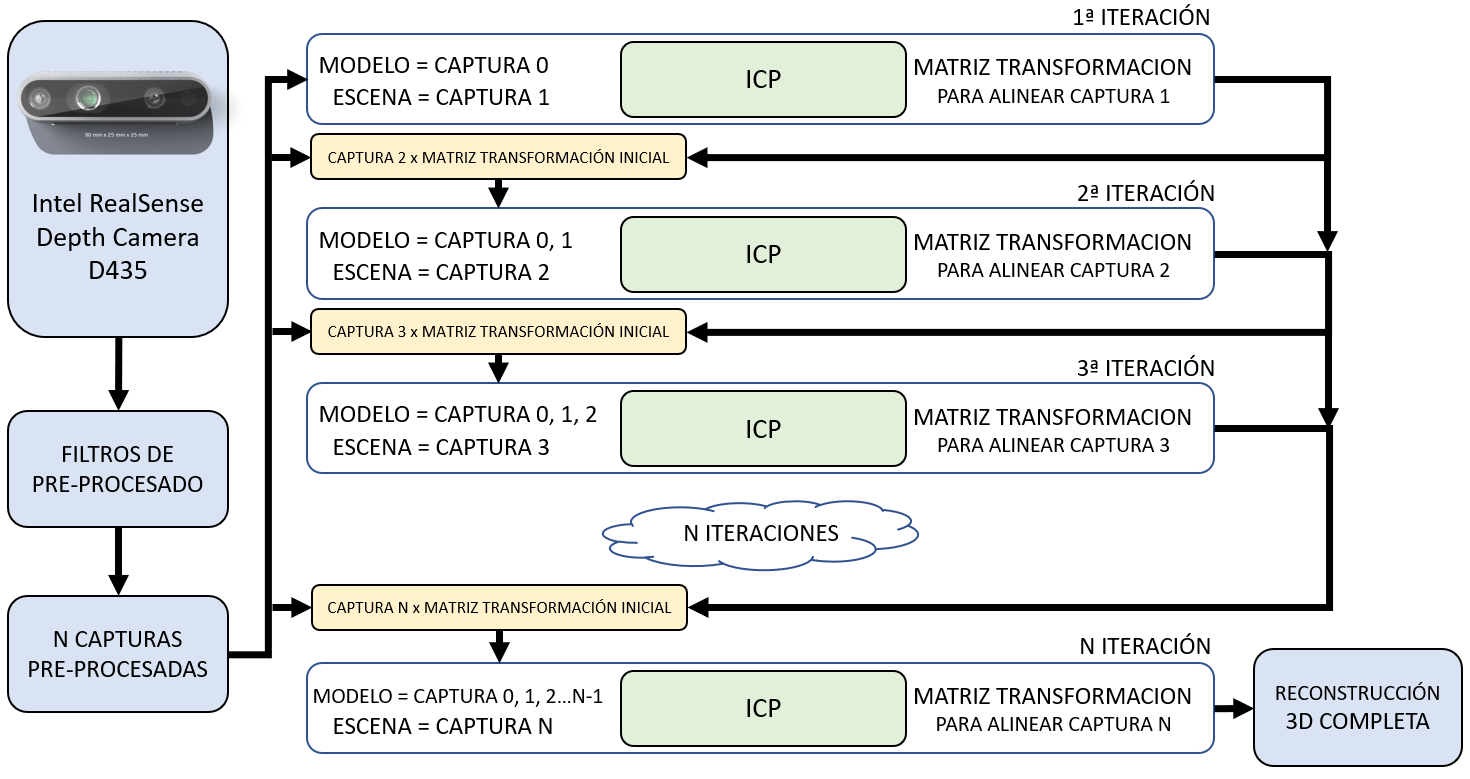
\includegraphics[width=\textwidth]{archivos/diagrama-acumulacion-matriz-transformacion.png}
    \caption{Diagrama de reconstrucción 3D acumulando matrices de transformación para cada nueva iteración.}
    \label{fig:diagrama-acumulacion-matriz-transformacion}
\end{figure}

\subsection{Posible refinamiento con CPD}

Como propuesta general, se puede hacer uso de un método de registro no rígido para corregir errores, como los producidos por el movimiento del cuerpo.
Concretamente se ha probado una pequeña implementación con el algoritmo \gls{cpd} explicado previamente en el apartado \ref{subsec:metodos-registro-no-rigido-cpd}.
La ventaja de este algoritmo es la posibilidad de utilizar el registro no rígido para corregir los errores de movimiento que se puedan haber producido durante la rotación 360º del cuerpo humano durante la fase de adquisición, ya que el cuerpo puede deformarse entre las capturas.
El algoritmo ha sido implementado de una manera similar a los otros dos, sin embargo no se contempla como solución final debido al largo tiempo de cómputo que emplea, no pudiendo proporcionar un resultado final.

\section{Post-procesado}

Tras finalizar la fase de registro y obtener el modelo final alineado y reconstruido, opcionalmente podemos utilizar la fase de post-procesado para aplicar unos filtros con la finalidad de reducir un poco el posible ruido que se haya podido generar durante la fase de registro.

Estos filtros serán el filtro ``Statistical Outlier Removal'' que se deshará de puntos atípicos lejanos a los bordes del modelo y el filtro de mediana, para aplanar y homogeneizar el modelo en sí.

\section{Análisis}

En esta última fase nos encontramos con una única nube de puntos, resultado de alinear todas las escenas con la primera nube de puntos de la fase de adquisición.

Esta nube de puntos la encontramos en un fichero con formato ``.ply'' que puede ser abierta por programas para visualizar nubes de puntos de modelos \gls{3d} como lo es MeshLab.
En la Figura \ref{fig:analisis-ejemplo-resultado} podemos ver un ejemplo de resultado en la fase de análisis.

\begin{figure}[h]
    \centering
    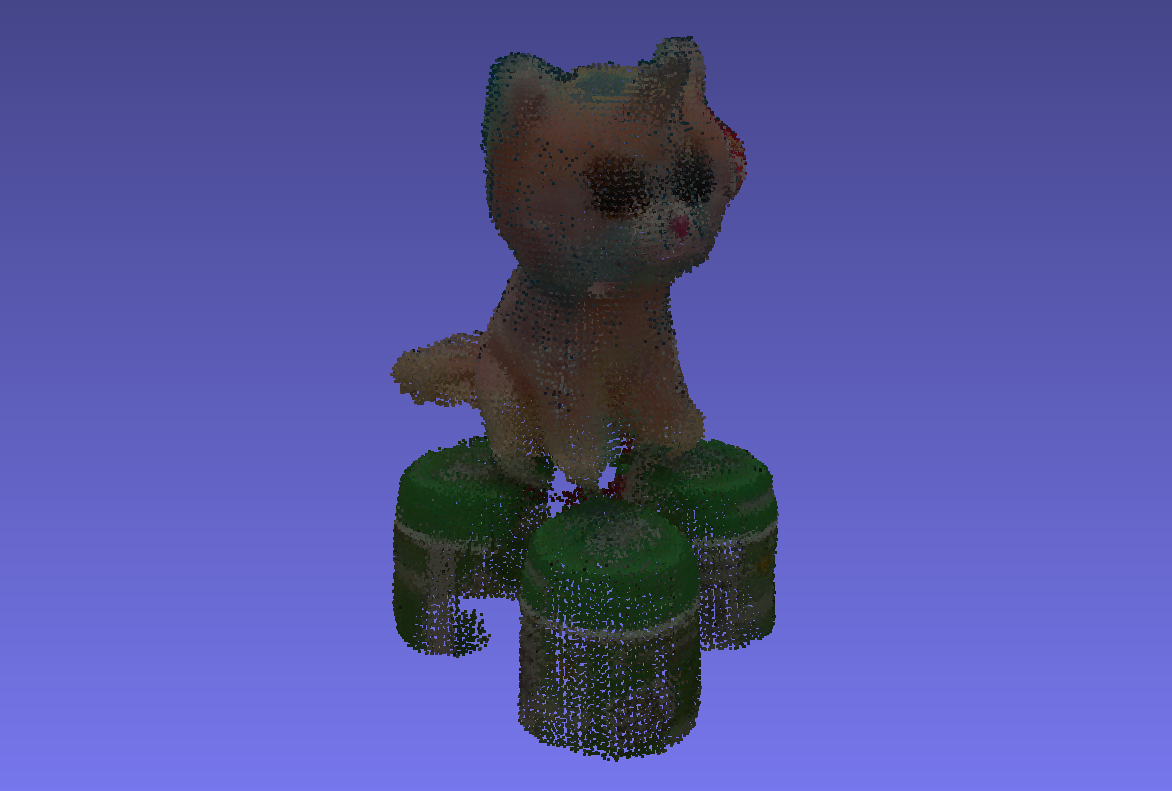
\includegraphics[width=\textwidth]{archivos/analisis-ejemplo-resultado.png}
    \caption{Ejemplo de modelo 3D en la fase de análisis.}
    \label{fig:analisis-ejemplo-resultado}
\end{figure}

Esta fase trata básicamente de visualizar el resultado para analizar posibles mejoras en la experimentación.
